\documentclass[
  captions=tableheading,
  bibliography=totoc, 
  titepage=firstiscover,
]{scrartcl}

\usepackage{blindtext} %neuer input

\usepackage{longtable} % Tabellen über mehrere Seiten

\usepackage[utf8]{inputenc} %neuer input

\usepackage{scrhack}

\usepackage[aux]{rerunfilecheck} %Warnung falls nochmal kompiliert werden muss

\usepackage{fontspec} %Fonteinstellungen

\recalctypearea{}

\usepackage[main=ngerman]{babel} %deutsche Spracheinstellung

\usepackage{ragged2e} %neuer input

\usepackage{amsmath, nccmath}

\usepackage{amssymb} %viele mathe Symbole

\usepackage{mathtools} %Erweiterungen für amsmath


\DeclarePairedDelimiter{\abs}{\lvert}{\rvert}
\DeclarePairedDelimiter{\norm}{\lVert}{\rVert}

\DeclarePairedDelimiter{\bra}{\langle}{\rvert}
\DeclarePairedDelimiter{\ket}{\lvert}{\rangle}

\DeclarePairedDelimiterX{\braket}[2]{\langle}{\rangle}{
#1 \delimsize| #2
}

\NewDocumentCommand \dif {m}
{
\mathinner{\symup{d} #1}
}


\usepackage[
  math-style=ISO,
  bold-style=ISO,
  sans-style=italic,
  nabla=upright,
  partial=upright,
  warnings-off={
    mathtools-colon,
    mathtools-overbracket,
  },
]{unicode-math}

\setmathfont{Latin Modern Math}
\setmathfont{XITS Math}[range={scr, bfscr}]
\setmathfont{XITS Math}[range={cal, bfcal}, StylisticSet=1]


\usepackage[
  locale=DE,
  separate-uncertainty=true,
  per-mode=reciprocal,
  output-decimal-marker={,},
]{siunitx}

\usepackage[autostyle]{csquotes} %richtige Anführungszeichen

\usepackage{xfrac}

\usepackage{float}

\floatplacement{figure}{htbp}

\floatplacement{table}{htbp}

\usepackage[ %floats innerhalb einer section halten
  section,   %floats innerhalb er section halten
  below,     %unterhalb der Section aber auf der selben Seite ist ok
]{placeins}

\usepackage[
  labelfont=bf,
  font=small,
  width=0.9\textwidth,
]{caption}

\usepackage{subcaption} %subfigure, subtable, subref

\usepackage{graphicx}

\usepackage{grffile}

\usepackage{booktabs}

\usepackage{microtype} %Verbesserungen am Schriftbild

\usepackage[
backend=biber,
]{biblatex}

\addbibresource{../lit.bib}

\usepackage[ %Hyperlinks im Dokument
  german,
  unicode,
  pdfusetitle,
  pdfcreator={},
  pdfproducer={},
]{hyperref}

\usepackage{bookmark}

\usepackage[shortcuts]{extdash}

%\usepackage{warpcol}

\usepackage{physics}
\allowdisplaybreaks

\begin{document}
    \title{Physik IV Übungsblatt 11}
    \author{  
    Tobias Rücker\\
    \texorpdfstring{\href{mailto:tobias.ruecker@tu-dortmund.de}{tobias.ruecker@tu-dortmund.de}
    \and}{,} 
    Paul Störbrock\\
    \texorpdfstring{\href{mailto:paul.stoerbrock@tu-dortmund.de}{paul.stoerbrock@tu-dortmund.de}}{}
    }
\maketitle
\center{\Large Abgabegruppe: \textbf{4H}}
\thispagestyle{empty}

\newpage
\tableofcontents
\thispagestyle{empty}
\newpage

\setcounter{page}{1}

\section{Aufgabe 1}
\begin{figure}[H]
    \centering
    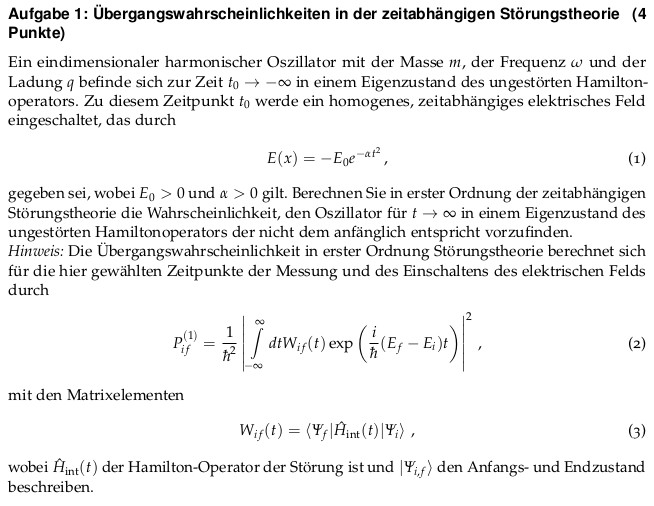
\includegraphics[width=\textwidth]{images/ex1.jpg}
\end{figure}
Bestimmung des Störungsteil des Hamilton-Operator:
\begin{align}
    q E(t,x) &= - \del{}{x} \phi \\
    \phi &= \int q E_0 e^{- \alpha t^2} \,\dif{x}\\
    &=q E_0 x e^{-\alpha t^2}\\
    \hat H _{int} (t) &= q E_0 \hat x e^{-\alpha t^2}\\
    \intertext{
        Bestimmung der Matrixelemente $W_{if}(t) $
    }
    \bra{\psi _f} q E_0 \hat x e^{- \alpha t^2} \ket{\psi _i}&= q E_0 e^{-\alpha t^2} \bra{\psi _f} \hat x \ket{\psi _i}  \\
    \intertext{
        Um die Wahrscheinlichkeit von einem Zustand i in einen beliebigen Zustand f
        zu bestimmen, wird die Formel 2 vom Blatt über alle f summiert.
    }
    \sum _{f, f \ne i} P_{if}^{(1)} &= \sum _{f, f \ne i} \frac{1}{\hbar ^2} \abs{ \int_{-\infty}^{\infty} \.\dif{t} q E_0 e^{-\alpha t^2} \bra{\psi _f} \hat x \ket{\psi _i} \exp \left( \frac{i}{\hbar} (E_f - E_i)t \right) }^2\\
    \intertext{
        Zwischenrechnung:
    }
    \hat x &= \sqrt{\frac{\hbar}{2m \omega}} (\hat a + \hat a ^\dagger)\\
    \bra{\psi _f} \sqrt{\frac{\hbar}{2m \omega}} (\hat a + \hat a ^\dagger) \ket{\psi _i}\\
    &= \sqrt{\frac{\hbar}{2m \omega}} (\bra{\psi _f} \hat a \ket{\psi _i} + \bra{\psi _f} \hat a ^{\dagger} \ket{\psi _i} )\\
    &= \sqrt{\frac{\hbar}{2m \omega}} (\sqrt{i} \delta _{f,i-1} + \sqrt{i+1} \delta _{f,i+1} )\\
    \intertext{
        Einsetzen in P und weiterrechnen
    }
    &= \sum _{f, f \ne i} \frac{1}{\hbar ^2} \abs{ \int_{-\infty}^{\infty} \,\dif{t} q E_0 \sqrt{\frac{\hbar}{2m \omega}} e^{-\alpha t^2} \exp \left( \frac{i}{\hbar} (E_f-E_i)t \right) (\sqrt{i} \delta _{f,i-1} + \sqrt{i+1} \delta _{f,i+1} ) }^2  \\
    &= \sum _{f, f \ne i} \frac{q^2 E_0^2}{2 \hbar m \omega}  \abs{\sqrt{i} \delta _{f,i-1} + \sqrt{i+1} \delta _{f,i+1} }^2 \abs{ \int_{-\infty}^{\infty} \,\dif{t} \exp \left(-\alpha t^2 \frac{i}{\hbar} (E_f-E_i)t \right)  }\\
    \intertext{
        quadratische Ergänzung und Substitution des Exponenten zum Lösen des Integrals
    }
    - \alpha t^2 + \underbrace{\frac{i}{\hbar} (E_f -E_i) }_{=C} t\\
    &= - \alpha \left(t^2 - \frac{C}{\alpha} t + \frac{C^2}{4\alpha ^2} - \frac{C^2}{4 \alpha ^2} \right)\\
    &= - \alpha \left( t- \frac{C}{2 \alpha} \right)^2 + \frac{C^2}{4 \alpha}\\
    u  &= t-\frac{C}{2 \alpha}\\
    \frac{\dif{u}}{\dif{t}}=1\\
    \intertext{weiter mit der Rechnung}
    &= \sum _{f, f \ne i} \frac{q^2 E_0^2}{2 \hbar m \omega} \abs{\sqrt{i} \delta _{f,i-1} + \sqrt{i+1} \delta _{f,i+1} }^2 \abs{\int_{-\infty}^{\infty} \,\dif{u} e^{\frac{c^2}{4\alpha} \exp (-\alpha u^2) } }^2\\
    &= \sum _{f, f \ne i} \frac{q^2 E_0^2}{2 \hbar m \omega} e^{\frac{C^2}{2\alpha}} \abs{\sqrt{i} \delta _{f,i-1} + \sqrt{i+1} \delta _{f,i+1} }^2 \abs{\sqrt{\frac{\pi}{\alpha}}}^2\\
    \intertext{
        Beim Auflösen der Summe bleiben nur die Elemente mit $f=i\pm 1$ übrig. Alle
        anderen verschwinden. Für $C^2$ ergibt sich dadurch.
    }
    C^2 &= -\frac{1}{\hbar ^2} (E_{i\pm 1} - E_i)^2 \\
    &= -\frac{1}{\hbar ^2} (i\pm 1 + \frac{1}{2}-i-\frac{1}{2} )^2 \hbar ^2 \omega ^2\\
    &= -\omega ^2\\
    \intertext{weiter}
    &= \frac{q^2 E_0^2 \pi}{2 \hbar m \omega \alpha} \exp \left(\frac{- \omega ^2}{2\alpha}\right) (2i+1)
\end{align}

\section{Aufgabe 2}
\begin{figure}[H]
    \centering
    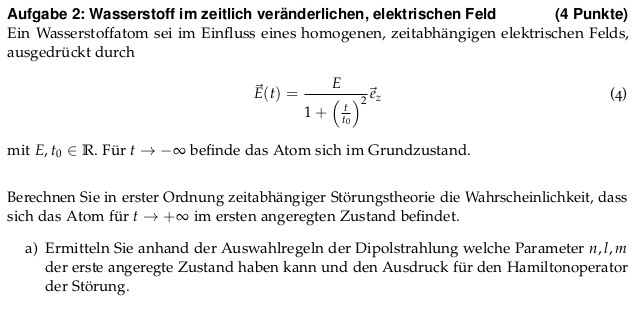
\includegraphics[width=\textwidth]{images/ex2a.jpg}
\end{figure}
\begin{figure}[H]
    \centering
    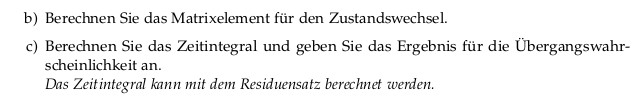
\includegraphics[width=\textwidth]{images/ex2b.jpg}
\end{figure}
\subsection{a)}
Der Grundzustand des Wasserstoffatoms wird durch den Zustand
\begin{align}
    \ket{\psi _{nlm} } &= \ket{\psi _{100}}.
\end{align}
Da wir in den ersten angeregten Zustand ist $n'=2$.\\
Die Wellenfunktion $\psi _{nlm} =R_{n,l} (r) \Theta _{l,m} (\theta) \Phi _{m} (\varphi) $
Aus dem 3. Faktor lässt sich eine Ausnahmeregel herleiten, da dieser nicht verschwinden darf
\begin{align}
    \Phi _m &= \frac{1}{\sqrt{2 \pi}} e^{im \varphi}\\
    \int_0^{2 \pi} \Phi ^* _{m'} \Phi _m &= \frac{1}{2 \pi} \int_0^{2 \pi} e^{i(-m'+m)\varphi} \,\dif{\varphi}\\
    &=
    \begin{cases}
        0 & m\ne m' \\
        1 & m = m'
    \end{cases}\\
    \intertext{
        Daraus folgt, dass $m' = 0$ sein muss.
        Die Ausnahmeregel wird dann so geschrieben
    }
    \Delta m = m'-m =0
\end{align}
Aus dem 2. Faktor lässt sich eine zweite Ausnahmeregel herleiten.
\begin{align}
    \Theta _{l,m} &= N_{l,m} P_l^m (\cos \theta)\\
    N_{l,m} &= \frac{2l+1}{2} (\frac{(l-\abs{m})!}{(l+ \abs{m})!})^{\frac{1}{2}} \\
    \int _0^{\pi} \Theta _{l',m'} \Theta _{l,m}&= N_{l' m} N_{l,m} \int_0^{\pi}  P_{l'}^m (\cos \theta)  P_l^m (\cos \theta) \cos \theta \sin \theta \,\dif{\theta} \\
    \intertext{
        in der letzten Zeile ist die erste Ausnahmeregel angewandt worden. 
        Substitution:
    }
    x = \cos \theta
    \intertext{
        weiter
    }
    &= N_{l' m} N_{l,m} \int_{-1}^{1} P_{l'}^m (x) x P_l^m (x) \,\dif{x}\\
    \intertext{
        Aus der Rekursionsformel
    }
    x P_l^m (x) &= \frac{l+m}{2l+1} P_{l-1}^m (x) - \frac{l+1-m}{2l+1} P_{l+1}^m (x)\\
    \intertext{
        ergibt sich die folgende Formel
    }
    &= N_{l',m} N_{l,m} \left(\frac{l+m}{2l+1} \int_{-1}^1 P_{l'}^m (x) P_{l-1}^m \dif{x} - \frac{l+1-m}{2l+1} \int_{-1}^1 P_{l'}^m P_{l+1}^m (x) \,\dif{x}   \right)
\end{align}
Dieser Term verschwindet nur für $l' =l \pm 1$ nicht.
Daraus ergibt sich die Ausnahmeregel\\
$\Delta l = \pm 1 $\\
Für das Wasserstoffatom ergibt sich, da der Grundzustand 0 ist, nur $l'=1$, da l nicht negativ sein kann.\\

Berechnung des Störungsanteil des Hamilton-Operators:

\begin{align}
    V &= \frac{-E}{1+\left( \frac{t}{t_0} \right)^2} \vec p \vec e _z 
    \intertext{
        wobei  das elektrische Dipolmoment ist
    }
    \hat H _{int} &= \frac{-eE}{1+\left( \frac{t}{t_0} \right)^2} z
\end{align}

\subsection{b)}
\begin{align}
    \frac{-eE}{1+\left( \frac{t}{t_0} \right)^2} \bra{\psi _{210}z \ket{\psi _{100}} }\\
    &= \alpha \int \,\dif{r^3} \psi _{210} z \psi _{100} \\
    &= \alpha \int \,\dif{r^3} R_{21}^* Y_{10}^* (\theta , \varphi) z Y_{00}(\theta, \varphi) R_{10}\\
    \alpha =\frac{-eE}{1+\left( \frac{t}{t_0} \right)^2}\\
    \intertext{
        Umschreiben in Kugelkoordinaten
    }
    z &= r \cos \theta \\
    \intertext{
        weiter mit der Hauptrechnung
    }
    &=\alpha \int \,\dif{r} R_{21}^* R_{10} \int \,\dif{\Omega} r^2 Y_{10}^* r \cos{\theta} Y_{00}\\
    \intertext{
        Definition der einzelnen Terme
    }
    Y_{00} &= \frac{1}{\sqrt{4 \pi}}\\
    Y_{10} &= \sqrt{\frac{3}{4 \pi}}\\
    Y_{00} \cos \theta &= \frac{1}{\sqrt{3}} Y_{10}\\
    R_{10} &= 2 e^{-\frac{r}{a_0}} \\
    R_{21} &= \frac{1}{1\sqrt{6}} e^{-\frac{r}{2 a_0}} \frac{r}{a_0}\\
    \rho &= \frac{r}{a_0} \\
    \frac{\dif{r}}{\dif{\rho}} = a_0\\
    \intertext{
        Die Funktionen für R und Y sind dabei der Vorlesung 29.05.2020 entnommen.
    }
    &= \alpha \int_0^{\infty} \dif{\rho} a_0^4 \rho ^4 \frac{1}{\sqrt{6}} e^{-\frac{3}{2} \rho} \frac{1}{\sqrt{3}} \int \dif{\Omega} Y_{10}^* Y_{10}\\
    \intertext{
        da Kugelflächenfkt. normiert sind
    }
    &= \alpha \frac{a_0^4}{\sqrt{18}} \int_0^{\infty} \dif{\rho} \rho ^4 e^{-\frac{3}{2} \rho}
    \intertext{
        Randterme werden verschwinden, da bei 0 das Polynom verschwindet und bei Unendlich die e-Funktion.
        Dadurch wird das Integral nach der mehrfachen partiellen Integration zu
    }
    \Rightarrow \int_0^{\infty} \dif{\rho} \rho ^4 e^{-\frac{3}{2} \rho} &= (-1)^4 (-\frac{2}{3})^4 4! \int_0^{\infty} e^{-\frac{3}{2}\rho} \dif{\rho}\\
    &=\frac{256}{81}\\
    \intertext{
        die -1 kommen aus dem zweiten Term partiellen Integration, der Bruch kommt aus der
        Integration der e-Funktion, die Fakultät aus der Ableitung des Polynoms
    }
    \Rightarrow \bra{\Psi _{210}}\hat H _{int} \ket{\Psi _{100}}&= \alpha \frac{a_0^4}{\sqrt{18}} \frac{256}{81} \\
\end{align}


\subsection{c)}
Aus der ersten Aufgabe
\begin{align}
    P_{if}^{(1)} &= \frac{1}{\hbar ^2} \abs{\int_{-\infty}^{\infty} \dif{t} W_{if}(t) \exp \left( \frac{i}{\hbar} (E_f - E_i)t \right) }^2\\
    P_{12}^{(1)} &= \frac{1}{\hbar ^2} \abs{\int_{-\infty}^{\infty}\dif{t} W_{12}(t) \exp \left( \frac{i}{\hbar} (E_2 - E_1)t \right) }^2\\
    W_{12} &=\alpha \frac{a_0^4}{\sqrt{18}} \frac{256}{81}\\
    E_2-E_1 &= (-\frac{1}{2^2}+\frac{1}{1^2}) E_{Ryd}\\
    &= \frac{3}{4} E_{Ryd}\\
    P_{12}^{(1)} &= \frac{1}{\hbar ^2} \abs{\int_{-\infty}^{\infty}\dif{t} \frac{(-qE)}{1+\left( \frac{t}{t_0} \right)^2} \frac{256 a_0^4 }{81 \sqrt{18}} \exp \left(\frac{i}{\hbar} \frac{3}{4} E_{Ryd} t \right) }^2
    \intertext{
        Substitution
    }
    \frac{t}{t_0} &= z \quad z \in \symbb{C}\\
    \frac{\dif{t}}{\dif{z}}&= t_0\\
    \intertext{
        weiter
    }
    &= \frac{q2 E^2 a_0^8}{18 } (\frac{256}{81})^2 \abs{t_0 \int_{C_r} \frac{\exp \left(\frac{i}{\hbar} \frac{3}{4} E_{Ryd} t_0 z \right)}{1+z^2} \,\dif{z} }^2\\
    &= \frac{q^2 E^2 a_0^8 t_0^2}{18} (\frac{256}{81})^2 \abs{2\pi i  \,\text{Res}(f,i)+ \,\text{Res}(f,-i) }^2\\
    \intertext{
        da $h'(\pm i)=(1+z^2)' \vert _{\pm i} \ne 0 $ ist, ist das Residuum
    }
    \text{Res} (f, \pm i) &= \frac{g(z)}{h'(z)} \vert _{\pm i}\\
    &= \frac{\exp \left(\frac{i}{\hbar} \frac{3}{4} E_{Ryd} t_0 z \right)}{2z} \vert _{\pm i}\\
    &=\frac{\exp \left(\mp \frac{3}{4\hbar} E_{Ryd} t_0 z \right)}{\pm 2i} \vert _{\pm i}\\
    \intertext{eingesetzt ergibt das}
    &= \frac{q^2 E^2 a_0^8 t_0^2\pi ^2}{18} (\frac{256}{81})^2 \abs{ \exp (\left(- \frac{3}{4\hbar} E_{Ryd} t_0 \right)) -\exp (\left(\frac{3}{4\hbar} E_{Ryd} t_0 \right)) }^2 \\ 
    &=  \frac{q^2 E^2 a_0^8 t_0^2\pi ^2}{18} (\frac{256}{81})^2 \abs{-2 \sinh \left( \frac{3}{4 \hbar} E_{Ryd} t_0 \right) }^2\\
    &=\frac{2q^2 E^2 a_0^8 t_0^2 \pi ^2}{9} (\frac{256}{81})^2 \abs{ \sinh \left( \frac{3}{4 \hbar} E_{Ryd} t_0 \right) }^2
\end{align}


\section{Aufgabe 3}
\begin{figure}[H]
    \centering
    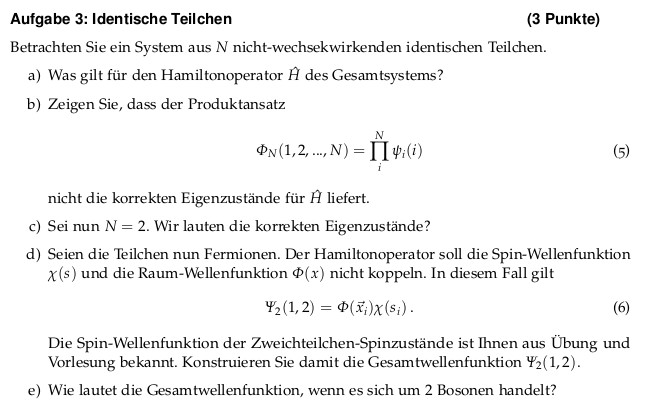
\includegraphics[width=\textwidth]{images/ex3.jpg}
\end{figure}
\subsection{a)}

     \flushleft{Der\;}\justifying Hamilton Operator ist symmetrisch unter Permutation. Das heißt, dass der
     Permutationsoperator $P$ und der Hamiltonoperator $H$ im Produkt vertauschbar sind:
     \begin{align}
        PH &= HP
        \intertext{
            \flushleft{Und,\;}\justifying dass diese kommutieren:
        }
        [P,H] &= 0
     \end{align}


\subsection{b)}


\subsection{c)}


\subsection{d)}


\subsection{e)}


\section{Aufgabe 4}
\begin{figure}[H]
    \centering
    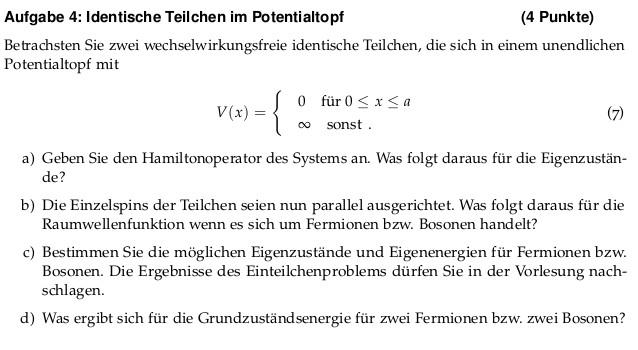
\includegraphics[width=\textwidth]{images/ex4.jpg}
\end{figure}

\subsection{a)}

\subsection{b)}

\subsection{c)}

\subsection{d)}


\end{document}